\documentclass[11pt,a4paper]{article}
\usepackage{fontspec}
\usepackage{bidi}
\newfontfamily\arabicfont[Script=Arabic,Scale=1.08]{Arial}
\setmainfont{Arial}
\usepackage{geometry}
\usepackage{graphicx}
\usepackage{booktabs}
\usepackage{float}
\usepackage{amsmath}
\usepackage{caption}
\usepackage{setspace}
\geometry{margin=2.4cm}
\captionsetup{font=small,labelfont=bf}
\setstretch{1.06}
\setlength{\parskip}{0.35em}
\setlength{\parindent}{0pt}
\setlength{\emergencystretch}{3em}

\begin{document}

\begin{center}
{\LARGE\bfseries \arabicfont\RL{تقرير ثنائي اللغة: تحليل درجات التقييم}}\par
\vspace{0.35em}
{\Large\bfseries Rapport bilingue : corrélations des scores, \LR{PCA} et \LR{K-means}}\par
\vspace{0.5em}
{\small 17 avril 2026 / \arabicfont\RL{17 أبريل 2026}}\par
\end{center}

\begin{RTL}
\section*{{\arabicfont\RL{1. البيانات والمتغيرات}}}
يعتمد هذا التقرير على النتائج المنفذة فعلياً في الدفتر التحليلي، ويغطي \textbf{63{,}871} إعلاناً تتوفر لها قيم كاملة في سبعة متغيرات من درجات التقييم. ويستهدف التحليل فهم البنية المشتركة بين هذه المتغيرات، واختزالها إلى أبعاد أكثر تركيباً، ثم توصيف المجموعات الرئيسة من الإعلانات داخل هذا الفضاء المختزل.
\end{RTL}

\begin{LTR}
\section*{1. Donn\'ees et variables}
Ce rapport repose sur les sorties effectivement ex\'ecut\'ees dans le notebook analytique et couvre \textbf{63,871} annonces disposant de valeurs compl\`etes pour sept variables de scores. L'objectif est d'identifier la structure commune de ces scores, de la r\'esumer par analyse factorielle, puis de d\'ecrire les grands profils d'annonces \`a l'aide d'un clustering.
\end{LTR}

\begin{RTL}
\section*{{\arabicfont\RL{2. مخطط سير العمل}}}
يوضح الشكل التالي تسلسل المعالجة، من ملف الإدخال إلى الجداول والرسوم النهائية المستخدمة في التقرير.
\end{RTL}

\begin{LTR}
\section*{2. Sch\'ema du workflow}
La figure suivante r\'esume la cha\^ine de traitement, depuis le fichier d'entr\'ee jusqu'aux tableaux et graphiques finaux utilis\'es dans le rapport.
\end{LTR}

\begin{figure}[H]
    \centering
    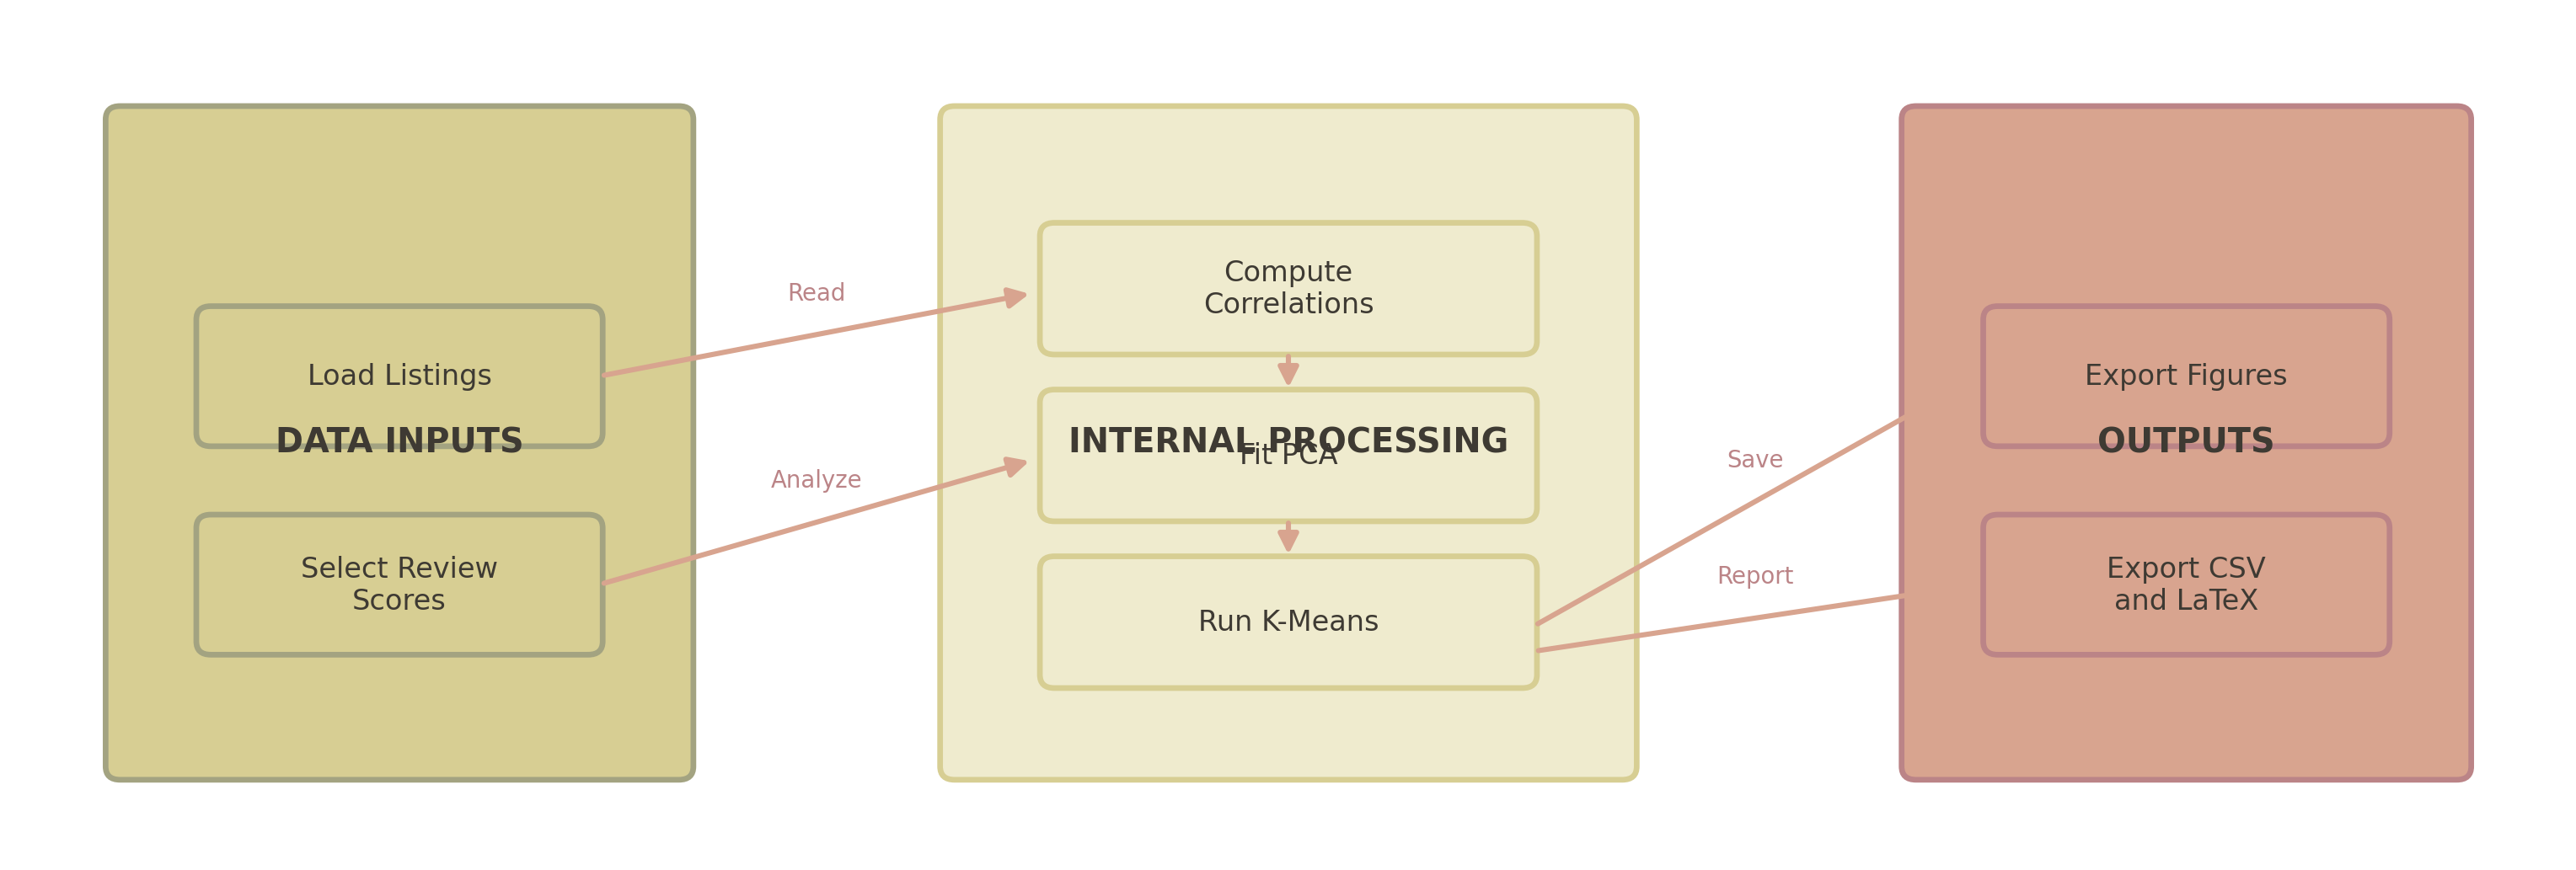
\includegraphics[width=0.96\textwidth]{p16_review_scores_correlation_pca_kmeans_mermaid.png}
    \caption{\arabicfont\RL{مخطط سير العمل التحليلي} / Workflow analytique du notebook}
    \label{fig:bilingual-workflow}
\end{figure}

\begin{RTL}
\section*{{\arabicfont\RL{3. الارتباطات الرئيسية}}}
تُظهر مصفوفة الارتباط أن جميع متغيرات التقييم تتحرك في الاتجاه نفسه تقريباً، ما يشير إلى وجود بعد عام للرضا. وأقوى العلاقات تظهر بين الدرجة العامة والدقة \((0.810)\)، وبين الدرجة العامة والقيمة مقابل السعر \((0.810)\)، ثم بين الدقة والقيمة \((0.771)\). أما الموقع فيبقى المتغير الأقل التصاقاً ببقية الأبعاد، وهو ما يبرر ظهوره لاحقاً كبعد أكثر استقلالاً في التحليل العاملي.
\end{RTL}

\begin{LTR}
\section*{3. Corr\'elations principales}
La matrice de corr\'elation montre que toutes les dimensions de notation varient globalement dans le m\^eme sens, ce qui sugg\`ere un facteur g\'en\'eral de satisfaction. Les liens les plus forts concernent la note globale avec la pr\'ecision \((0.810)\), la note globale avec la valeur \((0.810)\), puis la pr\'ecision avec la valeur \((0.771)\). La variable de localisation est la moins int\'egr\'ee au reste, ce qui annonce son r\^ole plus sp\'ecifique dans l'ACP.
\end{LTR}

\begin{table}[H]
\centering
\caption{\arabicfont\RL{مصفوفة الارتباط} / Matrice de corr\'elation}
\resizebox{\textwidth}{!}{%
\begin{tabular}{lrrrrrrr}
\toprule
 & note globale & pr\'ecision & propret\'e & check-in & communication & localisation & valeur \\
\midrule
note globale  & 1.000 & 0.810 & 0.734 & 0.647 & 0.721 & 0.504 & 0.810 \\
pr\'ecision   & 0.810 & 1.000 & 0.677 & 0.631 & 0.694 & 0.499 & 0.771 \\
propret\'e    & 0.734 & 0.677 & 1.000 & 0.512 & 0.545 & 0.420 & 0.672 \\
check-in      & 0.647 & 0.631 & 0.512 & 1.000 & 0.708 & 0.447 & 0.600 \\
communication & 0.721 & 0.694 & 0.545 & 0.708 & 1.000 & 0.461 & 0.669 \\
localisation  & 0.504 & 0.499 & 0.420 & 0.447 & 0.461 & 1.000 & 0.508 \\
valeur        & 0.810 & 0.771 & 0.672 & 0.600 & 0.669 & 0.508 & 1.000 \\
\bottomrule
\end{tabular}%
}
\end{table}

\begin{figure}[H]
    \centering
    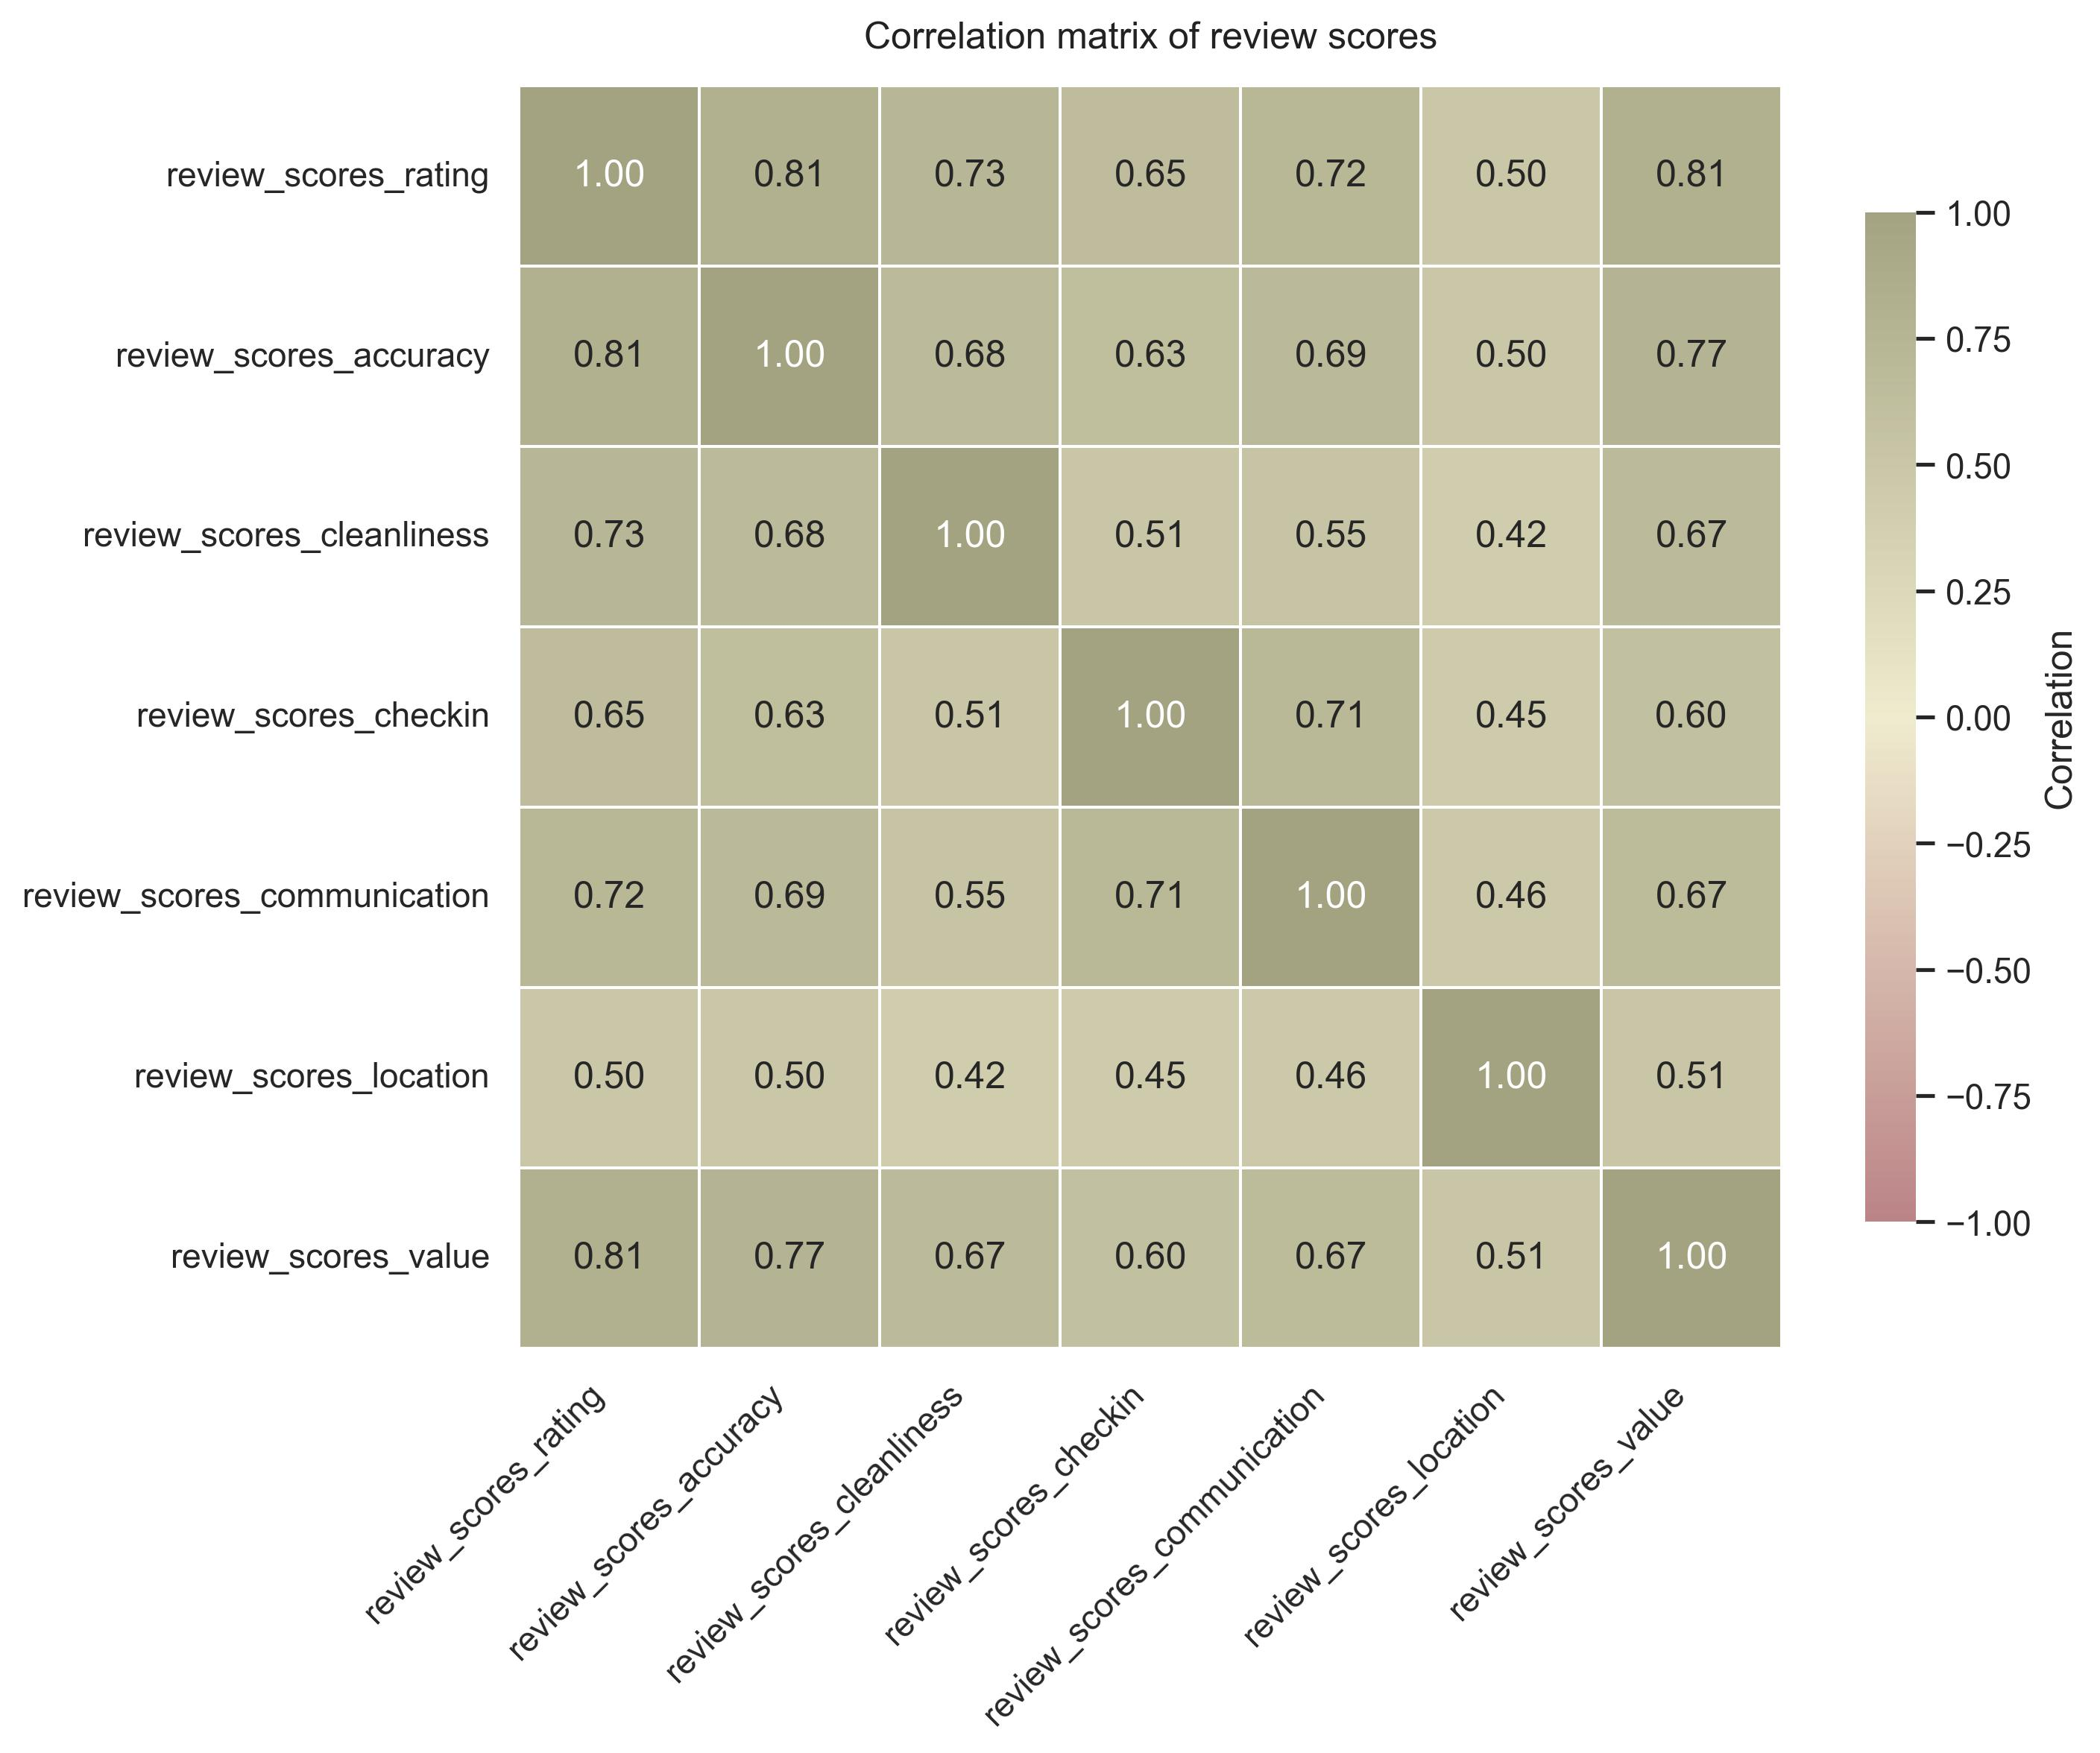
\includegraphics[width=0.9\textwidth]{p16_review_scores_corrplot.jpeg}
    \caption{\arabicfont\RL{الخريطة الحرارية للارتباطات} / Heatmap des corr\'elations}
\end{figure}

\begin{RTL}
\section*{{\arabicfont\RL{4. تحليل المكونات الرئيسية}}}
يُظهر \LR{PCA} أن المكون الأول يفسر \textbf{68.16\%} من التباين، بينما يرفع المكونان الأول والثاني النسبة التراكمية إلى \textbf{77.40\%}. هذا يعني أن الجزء الأكبر من المعلومات يتمحور حول بعد عام واحد يلتقط جودة التقييم الكلية. كما أن ارتفاع تحميل الموقع على \LR{PC2} \((0.752)\) يؤكد أن هذا المتغير يضيف بعداً تفسيرياً خاصاً لا يذوب بالكامل داخل المحور العام للرضا.
\end{RTL}

\begin{LTR}
\section*{4. Analyse en composantes principales}
L'ACP montre que la premi\`ere composante explique \textbf{68.16\%} de la variance, tandis que les deux premi\`eres composantes atteignent \textbf{77.40\%}. L'essentiel de l'information se concentre donc sur un axe g\'en\'eral de qualit\'e per\c cue. Le poids de la localisation sur \LR{PC2} \((0.752)\) confirme qu'il s'agit d'une dimension plus autonome que les autres scores.
\end{LTR}

\begin{table}[H]
\centering
\caption{\arabicfont\RL{التباين المفسر} / Variance expliqu\'ee}
\begin{tabular}{lrr}
\toprule
Composante & Part expliqu\'ee & Cumul \\
\midrule
\LR{PC1} & 0.6816 & 0.6816 \\
\LR{PC2} & 0.0925 & 0.7740 \\
\LR{PC3} & 0.0823 & 0.8564 \\
\LR{PC4} & 0.0491 & 0.9055 \\
\LR{PC5} & 0.0385 & 0.9440 \\
\LR{PC6} & 0.0323 & 0.9763 \\
\LR{PC7} & 0.0237 & 1.0000 \\
\bottomrule
\end{tabular}
\end{table}

\begin{table}[H]
\centering
\caption{\arabicfont\RL{تحميلات المتغيرات على أول محورين} / Loadings sur \LR{PC1} et \LR{PC2}}
\begin{tabular}{lrr}
\toprule
Variable & \LR{PC1} & \LR{PC2} \\
\midrule
note globale  & 0.916 & -0.131 \\
pr\'ecision   & 0.890 & -0.102 \\
propret\'e    & 0.795 & -0.212 \\
check-in      & 0.787 & 0.005 \\
communication & 0.836 & -0.044 \\
localisation  & 0.643 & 0.752 \\
valeur        & 0.881 & -0.081 \\
\bottomrule
\end{tabular}
\end{table}

\begin{figure}[H]
    \centering
    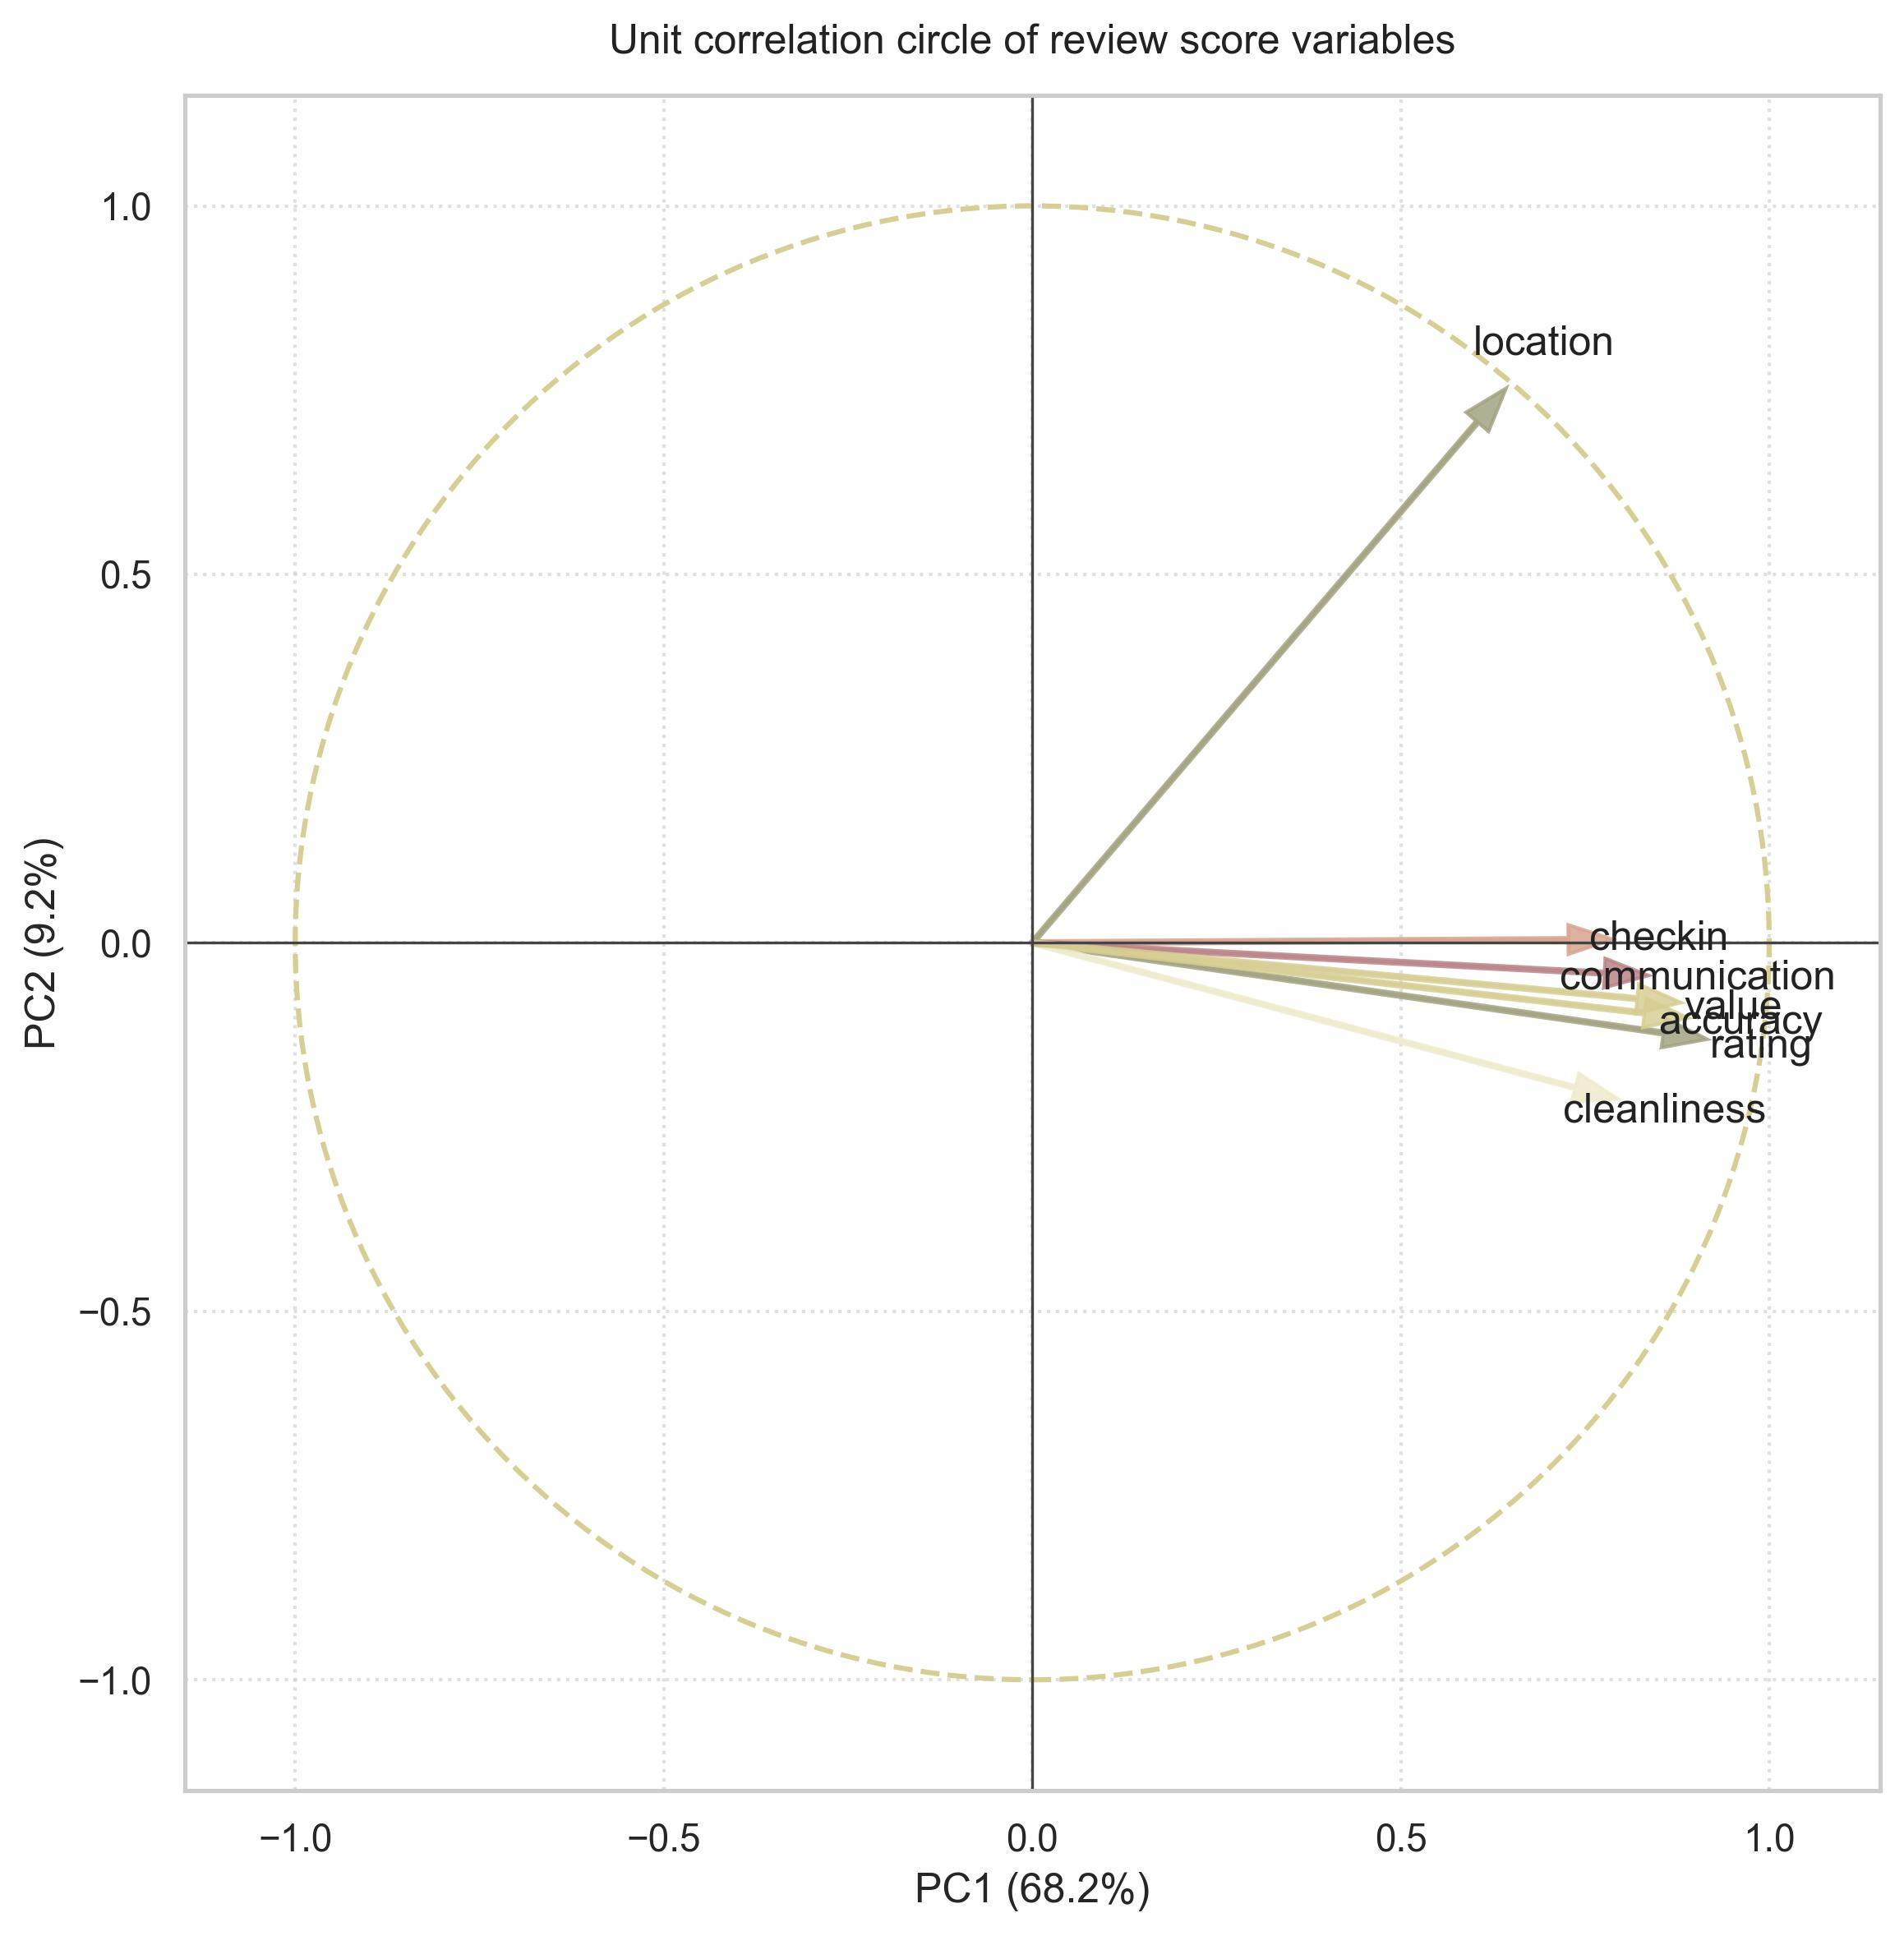
\includegraphics[width=0.8\textwidth]{p16_review_scores_pca_circle.jpeg}
    \caption{\arabicfont\RL{الدائرة الارتباطية} / Cercle des corr\'elations}
\end{figure}

\begin{RTL}
\section*{{\arabicfont\RL{5. التجميع بطريقة \LR{K-means}}}}
يشير اختيار \LR{k=2} إلى أن الفصل الأكثر وضوحاً في البيانات لا يكمن في تعدد أنماط متوازنة، بل في وجود مجموعة كبرى جداً وأخرى صغيرة ذات درجات أضعف بوضوح. وتضم المجموعة الأولى \textbf{60{,}789} إعلاناً، أي \textbf{95.17\%} من العينة، بينما تضم الثانية \textbf{3{,}082} إعلاناً فقط، أي \textbf{4.83\%}. كما أن تمركز المجموعة الثانية عند قيمة سالبة قوية على \LR{PC1} يدل على أن الفرق الأساسي بينها وبين الأغلبية هو انخفاض الجودة العامة المدركة.
\end{RTL}

\begin{LTR}
\section*{5. Clustering \LR{K-means}}
Le choix de \LR{k=2} indique que la s\'eparation la plus nette n'oppose pas plusieurs profils \`a poids comparable, mais une tr\`es grande masse d'annonces \`a une petite fraction plus faible sur l'axe g\'en\'eral de qualit\'e. Le cluster majoritaire rassemble \textbf{60,789} annonces, soit \textbf{95.17\%} de l'\'echantillon, contre \textbf{3,082} annonces \((4.83\%)\) pour le second. Le centre tr\`es n\'egatif du petit cluster sur \LR{PC1} montre que la diff\'erence principale tient avant tout \`a un niveau plus bas de satisfaction globale.
\end{LTR}

\begin{table}[H]
\centering
\caption{\arabicfont\RL{درجات السيليويت} / Scores de silhouette}
\begin{tabular}{rr}
\toprule
\LR{k} & Score \\
\midrule
2 & 0.7498 \\
3 & 0.5460 \\
4 & 0.4605 \\
5 & 0.4033 \\
6 & 0.4163 \\
\bottomrule
\end{tabular}
\end{table}

\begin{table}[H]
\centering
\caption{\arabicfont\RL{حجم المجموعات} / Taille des clusters}
\begin{tabular}{lrr}
\toprule
Cluster & Annonces & Part \\
\midrule
0 & 60{,}789 & 95.17\% \\
1 & 3{,}082 & 4.83\% \\
\bottomrule
\end{tabular}
\end{table}

\begin{table}[H]
\centering
\caption{\arabicfont\RL{مراكز المجموعات} / Centro\"ides}
\begin{tabular}{lrrr}
\toprule
Cluster & \LR{PC1} & \LR{PC2} & \LR{PC3} \\
\midrule
0 & 0.3532 & -0.0109 & 0.0064 \\
1 & -6.9455 & 0.2138 & -0.1252 \\
\bottomrule
\end{tabular}
\end{table}

\begin{figure}[H]
    \centering
    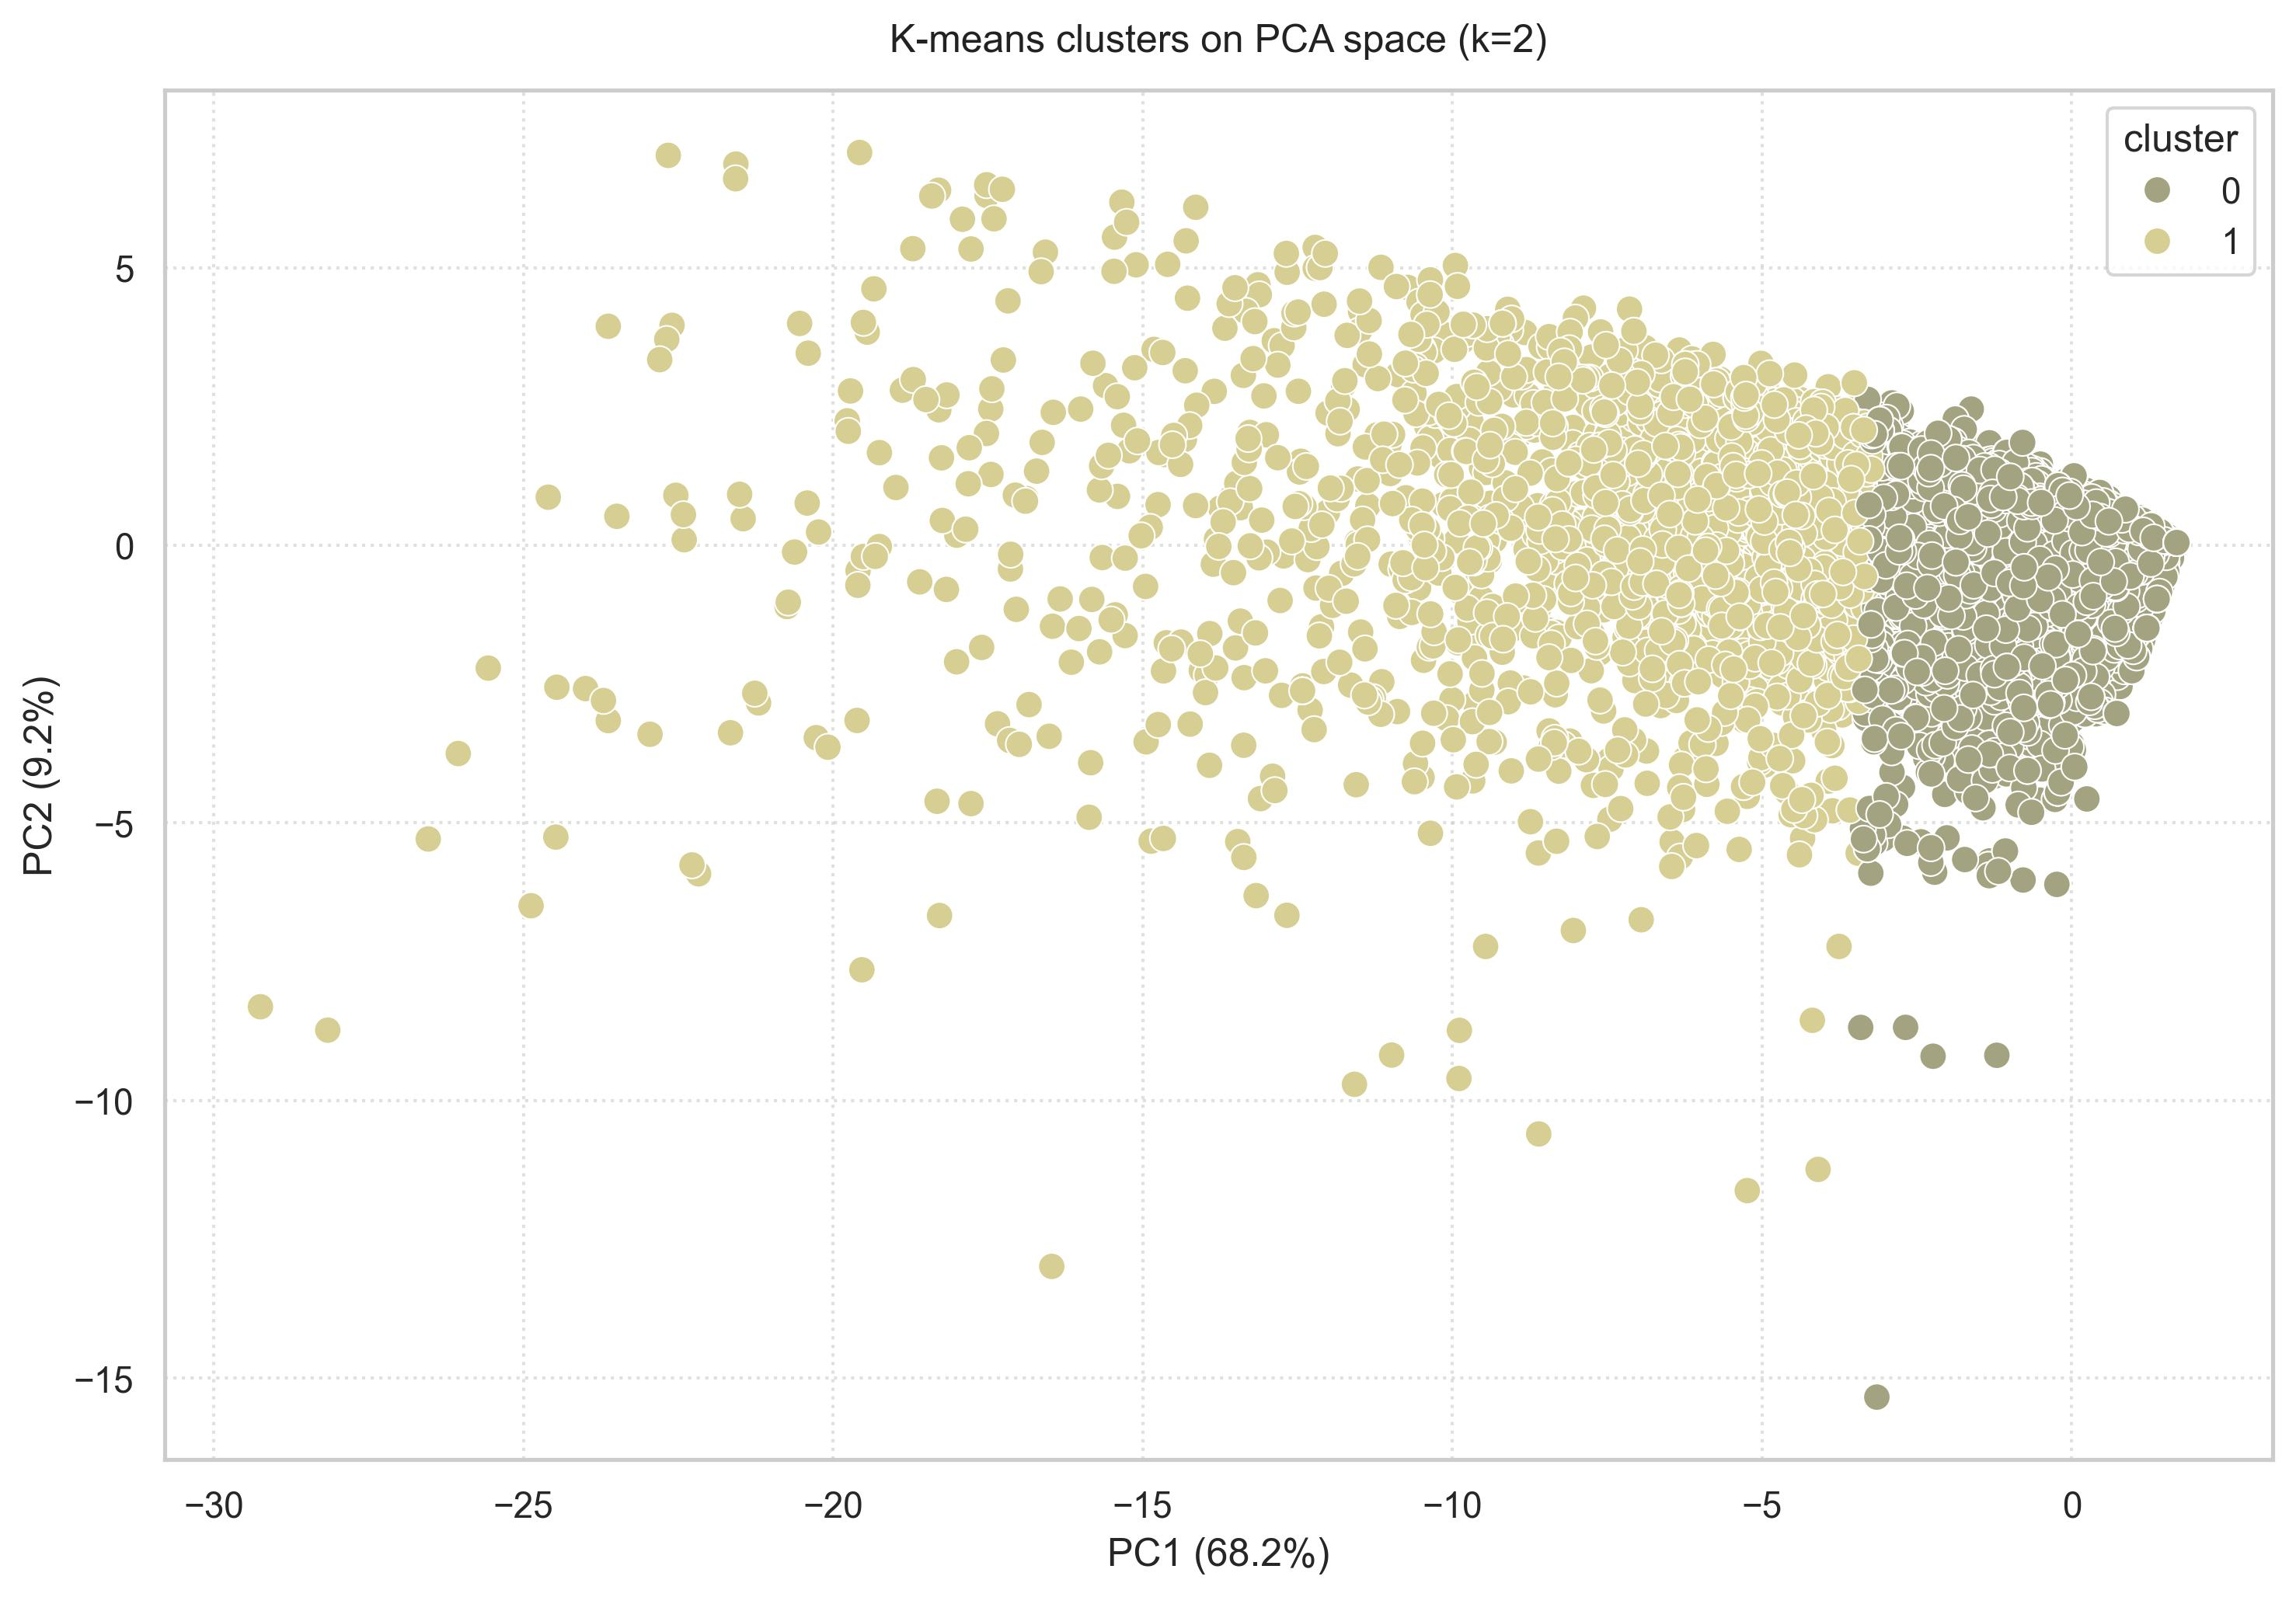
\includegraphics[width=0.92\textwidth]{p16_review_scores_kmeans_clusters.jpeg}
    \caption{\arabicfont\RL{تمثيل المجموعات في الفضاء العاملي} / Projection du clustering}
\end{figure}

\begin{RTL}
\section*{{\arabicfont\RL{6. خلاصة وتفسير}}}
تتفق النتائج على أن درجات التقييم في هذه البيانات تدور أساساً حول محور عام للرضا، مع احتفاظ الموقع بهامش من الاستقلال النسبي. كما أن التجميع يؤكد أن البنية التجريبية تحكمها في الأساس قطيعة بين أغلبية ذات تقييمات جيدة وأقلية صغيرة أضعف أداءً.
\end{RTL}

\begin{LTR}
\section*{6. Conclusion interpr\'etative}
L'ensemble des r\'esultats converge vers une lecture simple: les scores de notation sont domin\'es par un axe g\'en\'eral de satisfaction, tandis que la localisation conserve une part d'autonomie relative. Le clustering confirme que la structure empirique oppose surtout une large majorit\'e bien not\'ee \`a une petite minorit\'e plus fragile.
\end{LTR}

\begin{RTL}
\section*{{\arabicfont\RL{7. ملحق كربوني}}}
تستند القيم التالية إلى السجل الكربوني الفعلي المحفوظ بعد التنفيذ، وهي تمثل الحصيلة التشغيلية لهذا التحليل كما تم توثيقها داخل المشروع.
\end{RTL}

\begin{LTR}
\section*{7. Annexe carbone}
Les valeurs suivantes proviennent de la ligne effectivement enregistr\'ee dans le rapport carbone unifi\'e du projet. Elles correspondent donc \`a la trace op\'erationnelle r\'eelle de cette ex\'ecution.
\end{LTR}

\begin{table}[H]
\centering
\caption{\arabicfont\RL{الحصيلة الكربونية} / Bilan carbone de l'ex\'ecution}
\begin{tabular}{p{0.42\textwidth}p{0.32\textwidth}}
\toprule
Indicateur / \arabicfont\RL{المؤشر} & Valeur / \arabicfont\RL{القيمة} \\
\midrule
Notebook & \LR{p16 review-scores PCA K-means} \\
Observations trait\'ees & 63{,}871 \\
Date d'ex\'ecution & 2026-04-17 19:56:50 \\
Temps d'ex\'ecution & 364.81 s \\
Consommation \`electrique & 0.035468 \LR{kWh} \\
\'Emissions totales & 1.78 g \LR{eCO\textsubscript{2}} \\
\bottomrule
\end{tabular}
\end{table}

\end{document}